\documentclass[english]{article}

\usepackage{babel}
\usepackage{graphicx}
\usepackage{times}
\usepackage{pifont}
\usepackage[margin=1in]{geometry}
\usepackage{eurosym}
\usepackage{fancyhdr}
\usepackage{wrapfig}
\usepackage[hidelinks]{hyperref}

\pagestyle{fancy}
\fancyhf{}


%HEADER
%**************************************************************************************
\pagestyle{fancy}
\fancyhf{}
%**************************************************************************************
\lhead{Siemens Simatic}		 	 
\rhead{EFA0100 Control Engineering} 
\lfoot{EFA12SF}
\cfoot{\thepage}
\rfoot{Nikolai Arsenov, Alexey Tukalo}
%**************************************************************************************

\date{}
\setlength\parindent{0pt}

\begin{document}

\title{\vspace{2in}Siemens Simatic\\
\small for Control Engineering\\
\vspace{0.5in}
\includegraphics{savonia.jpg}}

\nopagebreak
\maketitle


\vspace{3in}

\author{
\begin{flushright}
Nikolai Arsenov, Alexey Tukalo,\\
EFA12SF,\\
Information Technology,\\
Savonia University of Applied Sciences
\end{flushright}
}

\date{\today}
\thispagestyle{empty}

\newpage
\setcounter{page}{1}
\setcounter{tocdepth}{2}
\tableofcontents

\newpage

%MAIN CONTENT ******************************************************************************************************************

\section{Siemens}
\begin{wrapfigure}{l}{0.5\textwidth}
  \begin{center}
    
\includegraphics[width=0.48\textwidth]{SiemensSimantic/Siemens_AG}
  \end{center}
  \caption{The logo of Siemens}
\end{wrapfigure}
Siemens AG is the largest engineering company in Europe. The principal divisions of the company are Industry, Energy, Healthcare, and Infrastructure \& Cities, which represent the main activities of the company. The company is a prominent maker of medical diagnostics equipment and its medical health-care division, which generates about 12 percent of the company's total sales, is its second-most profitable unit, after the industrial automation division.\\


Siemens and its subsidiaries employ approximately 349,000 people across nearly 190 countries and reported global revenue of approximately \euro 75 billion in 2013. The company has been the subject of a number of controversies in its history.

\section{Simatic}

\begin{wrapfigure}{r}{0.5\textwidth}
  \begin{center}
    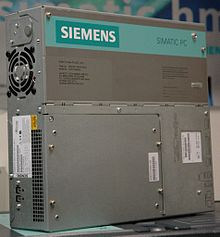
\includegraphics[width=0.4\textwidth]{SiemensSimantic/220px-Boxpc627}
  \end{center}
  \caption{Siemens Simatic IPC}
\end{wrapfigure}

SIMATIC is the name of an automation system which was developed by the German company Siemens. The automation system controls machines used for industrial production. This system makes it possible for machines to run automatically. Depending on the needed function of the machine you have to upload the right program on your Simatic unit. This unit is kept in a control cabinet near the machine.\\


The Simatic contains two main types of products: Software and Hardware solutions.
\subsection{Software}
SIMATIC WinCC is a supervisory control and data acquisition (SCADA) and human-machine interface (HMI) system from Siemens.
\subsubsection{SCADA} 
System control and data acquisition - is a system operating with coded signals over communication channels so as to provide control of remote equipment or collect data in real time and show an information about the monitoring object. SCADA systems are used to monitor and control physical processes involved in industry and infrastructure on a large scale and over long distances. 
A SCADA system usually consists of the following subsystems:
\begin{itemize}
\item Drivers, servers or IO - programs that provide communication with SCADA industrial controllers, counters, ADC and other input and output devices.
\item Real-time system - a program that provides the processing of data within a certain time cycle with the priorities.
\item Human-Machine Interface (HMI) - a tool that provides data about the process to a man operator, that provides to the human operator to control the process and to manage it.
\item Graphic Design program for the development of man-machine interface.
\item Logic control system - a program that provides execution of user programs (scripts) logic control in SCADA-system. Set of editors for its development.
\item Real-time database - a program that ensures the preservation of the history of the process in real time.
\item Alarm Management System - a program that provides automatic control of technological developments, to classify them in the category of normal, warning or alarm, and event handling by the operator or a computer.
\item Report Generator - program, which provides creating custom reports on technological developments. Set of editors for their development.
\item External interfaces - standard communication interfaces between SCADA and other applications. Typically, OPC, DDE, ODBC, DLL, etc.
\end{itemize}
WinCC is written for the Microsoft Windows operating system. It uses Microsoft SQL Server for logging and comes with a VBScript and ANSI C application programming interface.\\

SIMATIC WinCC in the Totally Integrated Automation Portal (TIA Portal) is part of a new, integrated engineering concept which offers a uniform engineering environment for programming and configuration of control, visualization and drive solutions. It is one software for all HMI tasks. SIMATIC WinCC V7 is still available for more complex applications with Plant Intelligence solutions or redundant architectures, while WinCC Open Architecture addresses solutions with highly customer-specific adaptation requirements, including on non-Windows platforms. 
\paragraph{Benefits}
\begin{itemize}
\item Innovative configuration interface based on the latest software technologies.
\item Comprehensive library concept for user-definable objectsand faceplates.
\item Intelligent tools for graphical configuration and mass data handling.
\end{itemize}

Compared to WinCC flexible, which has set the standards in engineering for years, configuration efficiency has been further increased, particularly if further TIA components such as the SIMATIC S7 Controller are part of the automation solution. The perfect interaction with STEP 7 in the TIA Portal prevents multiple entries and guarantees consistent data management at all times.

\subsubsection{Simatic Step 7}
 The software from Siemens for the development of automation systems based on programmable logic controllers (PLC) Simatic S7-300 / S7-400 / M7 / C7 and WinAC. For Simatic S7-200 there is its own product STEP 7 MicroWin. The software has a Multilanguage pack for an interface (English, German, French, Italian, Spanish and Russian). With this program, an operator can do the set of work to create or service the automatic system based on Simatic PLC.\\ 

\paragraph{STEP 7} utility works with a project, it allows configuration PLC and network in the industry. STEP 7 software significantly boosts efficiency in all of your automation tasks. Whether for configuring hardware, establishing communications, programming, testing, commissioning and service, documentation and archiving, or operational and/or diagnostic functions, the software sets the benchmark in its field.\\

An integrated program editor performs the controller’s programming in three main languages:
\begin{itemize}
\item LAD - Language ladder
\item FBD - Function block diagram language
\item STL - Language Instruction List\\\\
And additional languages:
\item SCL - structured control language, syntax close to Pascal
\item GRAPH 7 - language management process sequence
\item HiGraph 7 - language-based control of the state graph of the system
\item SFC - the language of state diagrams
\end{itemize}

Ability to monitor the current state of the program that is available using any programming language, provides not only debugging software, but also troubleshoot the equipment in the connected devices, even if it has no diagnostic tools.


\subsection{Hardware}
Simatic hardware contain two main types of devices: Industrial PCs and PLC.
\subsubsection{Industrial PC}
An industrial PC is an x86 PC-based computing platform for industrial applications.\\

Industrial PCs offer different features than consumer PCs in terms of reliability, compatibility, expansion options and long-term supply.\\

Industrial PCs are typically characterized by being manufactured in lower volumes than home or office PCs. A common category of industrial PC is the 19-inch rackmount form factor. Industrial PCs typically cost considerably more than comparable office style computers with similar performance. Single-board computers and backplanes are used primarily in Industrial PC systems. However, the majority of industrial PCs are manufactured with COTS motherboards.
\subsubsection{PLC}
A programmable logic controller is a digital computer used for automation of typically industrial electromechanical processes, such as control of machinery on factory assembly lines, amusement rides, or light fixtures. PLCs are used in many industries and machines.\\

The main principle of the PLC is in handing the signals from the connected sensors and distribute command's signals through output modules from the application to the actuators.  
\paragraph{Simantic S7-200}
is designed for building automation systems of low and medium complexity. The main features of the controller are:
\begin{itemize}
\item Simple in an installation, programming and maintenance.
\item Relatively cheap
\item Compact
\item Solution for simple and relatively complex tasks
\item Works autonomously or as intelligent slave systems Distributed IO.
\end{itemize}
The controller is used in an automation of small systems, like single machine-tools, purification systems, automatic gates, lifts, conveyor lines.
\paragraph{Simantic S7-300}
\begin{wrapfigure}{r}{0.5\textwidth}
  \begin{center}
    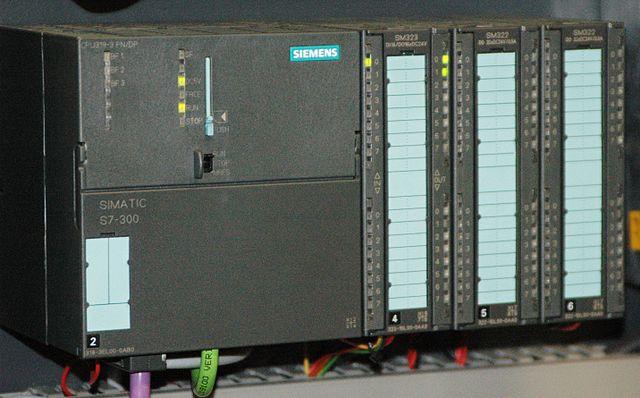
\includegraphics[width=0.4\textwidth]{SiemensSimantic/640px-S7300}
  \end{center}
  \caption{Simatic S7-300}
\end{wrapfigure}
an average performance PLC family of controllers developed by Siemens AG. It has several advantages  against S7-200:

\begin{itemize}
\item Advanced modular structure
\item Local and distributed IO
\item Wide range of interfaces (MPI, PROFInet, AS-i, BACnet, MODBUS TCP)
\item Support at the operating system level functions providing work in real time, hardware interrupts,  processing hardware and software errors
\item Scalable in case of modernization
\end{itemize}
A small factory or some unites of big one for example assembling line can be managed by S7-300.

\paragraph{Simantic S7-400}
 is series of programmable logic controllers for building automation systems of medium and high complexity. It contains all the features of S7-300, but more flexible and suitable for really complex projects. Can be used as a main control system for whole factory.

\paragraph{Simantic S7-1200 and S7-1500}
the Brand NEW solutions for simple and complex automation. They will replace S7-200, S7-300 and S7-400 soon. It realised on 2012 as totally new step in PLC world. 1200 should replace 200 and 1500 will store the place of 300 and 400.
\subsection{Features}
The main advantages of the solution are:
\begin{itemize}
\item Visualization of a technical process (Graphic Designer)
\item Configuration of micro controllers connections from different manufacturers (Tag Management)
\item Data acquisition report system (Report Designer)
\item Possibilities to work with other applications using SQL, ODBS, OLE interfaces
\item Redundancy - duplication of critical components or functions of a system, to  increase reliability  of the system (backup, fail-safe)
\item Compatible with MS SQL Server and Windows
\item Great opportunities using ActiveX
\item Simatic Step 7 utility
\end{itemize}

Redundancy is the duplication of critical components or functions of a system with the intention of increasing reliability of the system, usually in the form of a backup or fail-safe
\newpage
\section{References}
\begin{small}

\begin{enumerate}
\item  \href{http://iadt.siemens.ru/assets/files/infocenter/catalogs_and_brochures/as/ProductInfo/07_WinCC_V72_r.pdf}{WinCC doc.}
\item \href{http://w3.siemens.com/mcms/simatic-controller-software/en/step7/Pages/Default.aspx}{Step 7 doc.}
\item \href{http://docs.exdat.com/docs/index-35940.html}{Automation– and Drive Technology-SCE}
\item \href{http://en.wikipedia.org/wiki/SCADA}{Wikipedia - SCADA}
\item \href{http://en.wikipedia.org/wiki/WinCC}{Wikipedia - WinCC}
\item \href{https://ru.wikipedia.org/wiki/Simatic}{Wikipedia - Simatic}
\item \href{http://en.wikipedia.org/wiki/Industrial_PC}{Wikipedia - Industrial PC}
\item \href{https://ru.wikipedia.org/wiki/Simatic_S7-200}{Wikipedia - Simatic S7-200}
\item \href{https://ru.wikipedia.org/wiki/Simatic_S7-300}{Wikipedia - Simatic S7-300}
\item \href{https://ru.wikipedia.org/wiki/Simatic_S7-400}{Wikipedia - Simatic S7-400}
\end{enumerate}
\begin{flushright}
[\date{\today}]
\end{flushright}
\end{small}

\end{document}

